%%%%%%%%%%%%%%%%%%%%%%%%%%%%%%%%%%%%%%%%%
% Programming/Coding Assignment
% LaTeX Template
%
% This template has been downloaded from:
% http://www.latextemplates.com
%
% Original author:
% Ted Pavlic (http://www.tedpavlic.com)
%
% Note:
% The \lipsum[#] commands throughout this template generate dummy text
% to fill the template out. These commands should all be removed when 
% writing assignment content.
%
% This template uses a Perl script as an example snippet of code, most other
% languages are also usable. Configure them in the "CODE INCLUSION 
% CONFIGURATION" section.
%
%%%%%%%%%%%%%%%%%%%%%%%%%%%%%%%%%%%%%%%%%

%%%%%%%%%%%%%%%%%%%%%%%%%%%%%%%%%%%%%%%%%%%%%%
% Modified by George Z. Zachos
% on March 28, 2017 for the Parallel Systems
% and Programming course @cse.uoi.gr
%%%%%%%%%%%%%%%%%%%%%%%%%%%%%%%%%%%%%%%%%%%%%%

%----------------------------------------------------------------------------------------
%	PACKAGES AND OTHER DOCUMENT CONFIGURATIONS
%----------------------------------------------------------------------------------------

\documentclass{article}

\usepackage{fancyhdr} % Required for custom headers
\usepackage{lastpage} % Required to determine the last page for the footer
\usepackage{extramarks} % Required for headers and footers
\usepackage[usenames,dvipsnames]{xcolor} % Required for custom colors
\usepackage{graphicx} % Required to insert images
\usepackage{listings} % Required for insertion of code
\usepackage{courier} % Required for the courier font

% Margins
\topmargin=-0.45in
\evensidemargin=0in
\oddsidemargin=0in
\textwidth=6.5in
\textheight=9.0in
\headsep=0.25in

\linespread{1.1} % Line spacing

% Set up the header and footer
\pagestyle{fancy}
\lhead{\hmwkAuthorName} % Top left header
\chead{\hmwkClass: \hmwkTitle} % Top center head
\rhead{\firstxmark} % Top right header
\lfoot{\lastxmark} % Bottom left footer
\cfoot{} % Bottom center footer
\rfoot{Page\ \thepage\ of\ \protect\pageref{LastPage}} % Bottom right footer
\renewcommand\headrulewidth{0.4pt} % Size of the header rule
\renewcommand\footrulewidth{0.4pt} % Size of the footer rule

%\setlength\parindent{0pt} % Removes all indentation from paragraphs

%----------------------------------------------------------------------------------------
%	CODE INCLUSION CONFIGURATION
%----------------------------------------------------------------------------------------

\definecolor{MyDarkGreen}{rgb}{0.0,0.4,0.0} % This is the color used for comments
\lstloadlanguages{C}
\lstset{language=C,
%         commentstyle=\color{magenta}\itshape,
        morekeywords={pthread_t, pthread_cond_t, pthread_mutex_t},
%         keywordstyle=\color{blue},
%         emphstyle=\color{red},
        breaklines,
        basicstyle=\ttfamily,
        stringstyle=\color{magenta},
%         identifierstyle=\color{cyan}
        frame=single, % Single frame around code
        basicstyle=\ttfamily, % Use small true type font
        showstringspaces=false, % Don't put marks in string spaces
        tabsize=5, % 5 spaces per tab
%         morecomment=[l][\color{Blue}]{...}, % Line continuation (...) like blue comment
        numbers=left, % Line numbers on left
        firstnumber=0, % Line numbers start with line 0
        numberstyle=\small\color{Blue}, % Line numbers are blue and small
        stepnumber=1 % Line numbers go in steps of 1
}

% Creates a new command to include a perl script, the first parameter is the filename of the script (without .pl), the second parameter is the caption
\newcommand{\cscript}[2]{
\begin{itemize}
\item[]\lstinputlisting[caption=#2,label=#1]{#1.c}
\end{itemize}
}

\def\code#1{\texttt{#1}}
%----------------------------------------------------------------------------------------
%	DOCUMENT STRUCTURE COMMANDS
%	Skip this unless you know what you're doing
%----------------------------------------------------------------------------------------

% Header and footer for when a page split occurs within a problem environment
\newcommand{\enterProblemHeader}[1]{
\nobreak\extramarks{#1}{#1 continued on next page\ldots}\nobreak
\nobreak\extramarks{#1 (continued)}{#1 continued on next page\ldots}\nobreak
}

% Header and footer for when a page split occurs between problem environments
\newcommand{\exitProblemHeader}[1]{
\nobreak\extramarks{#1 (continued)}{#1 continued on next page\ldots}\nobreak
\nobreak\extramarks{#1}{}\nobreak
}

\setcounter{secnumdepth}{0} % Removes default section numbers
\newcounter{homeworkProblemCounter} % Creates a counter to keep track of the number of problems

\newcommand{\homeworkProblemName}{}
\newenvironment{homeworkProblem}[1][Problem \arabic{homeworkProblemCounter}]{ % Makes a new environment called homeworkProblem which takes 1 argument (custom name) but the default is "Problem #"
\stepcounter{homeworkProblemCounter} % Increase counter for number of problems
\renewcommand{\homeworkProblemName}{#1} % Assign \homeworkProblemName the name of the problem
\section{\homeworkProblemName} % Make a section in the document with the custom problem count
\enterProblemHeader{\homeworkProblemName} % Header and footer within the environment
}{
\exitProblemHeader{\homeworkProblemName} % Header and footer after the environment
}

\newcommand{\problemAnswer}[1]{ % Defines the problem answer command with the content as the only argument
\noindent\framebox[\columnwidth][c]{\begin{minipage}{0.98\columnwidth}#1\end{minipage}} % Makes the box around the problem answer and puts the content inside
}

\newcommand{\homeworkSectionName}{}
\newenvironment{homeworkSection}[1]{ % New environment for sections within homework problems, takes 1 argument - the name of the section
\renewcommand{\homeworkSectionName}{#1} % Assign \homeworkSectionName to the name of the section from the environment argument
\subsection{\homeworkSectionName} % Make a subsection with the custom name of the subsection
\enterProblemHeader{\homeworkProblemName\ [\homeworkSectionName]} % Header and footer within the environment
}{
\enterProblemHeader{\homeworkProblemName} % Header and footer after the environment
}

%----------------------------------------------------------------------------------------
%	NAME AND CLASS SECTION
%----------------------------------------------------------------------------------------

\newcommand{\hmwkTitle}{Homework \#3} % Assignment title
\newcommand{\hmwkDueDate}{Monday,\ June\ 12,\ 2017} % Due date
\newcommand{\hmwkClass}{MYE023} % Course/class
\newcommand{\hmwkClassTime}{} % Class/lecture time
\newcommand{\hmwkClassInstructor}{Vassilios V. Dimakopoulos} % Teacher/lecturer
\newcommand{\hmwkAuthorName}{George Z. Zachos} % Your name

%----------------------------------------------------------------------------------------
%	TITLE PAGE
%----------------------------------------------------------------------------------------

\title{
\vspace{2in}
\textmd{\textbf{\hmwkClass:\ \hmwkTitle}}\\
\normalsize\vspace{0.1in}\small{Due\ on\ \hmwkDueDate}\\
\vspace{0.1in}\large{\textit{\hmwkClassInstructor}}
\vspace{3in}
}

\author{\textbf{\hmwkAuthorName}}
\date{June 12, 2017} % Insert date here if you want it to appear below your name

%----------------------------------------------------------------------------------------

\setcounter{secnumdepth}{3}

\begin{document}

\maketitle

%----------------------------------------------------------------------------------------
%	TABLE OF CONTENTS
%----------------------------------------------------------------------------------------

\newpage
\tableofcontents
\newpage


%+----------------------------------------------------------+
%|                                                          |
%|          EXERCISE #1                                     |
%|                                                          |
%+----------------------------------------------------------+

\section{Exercise \#1}

\subsection{About}
This exercise is about the multiplication of integer $N$x$N$ arrays using \texttt{MPI} and
strip-partitioning. During strip-partitioning, only the \underline{outermost} for-loop of
the serial calculation is parallelized. The purpose of this exercise is to time the matrix
multiplication and observe how altering the number of \texttt{MPI} nodes\footnote{and
consequently the number of \texttt{MPI} processes} will affect execution time and what
amount of this time is spent in communications.

\subsection{Experiment details}
During this experiment, \texttt{MPI} node number takes value in \{2, 4, 8\}, 4 \texttt{MPI}
processes run in each node and array size is 1024x1024.

\subsubsection{System Specifications}
The experiments were conducted on a cluster of Dell OptiPlex 7020s connected via Ethernet
Local Area Network (LAN):
\begin{itemize}
 \item CPU: Intel\textregistered \ Core\texttrademark \ i5-4590 CPU @ 3.30GHz (64 bit)
 \item RAM: 2 DIMMs x4GiB @ 1600MHz DDR3
 \item Cache line size: 64B (in all levels)
 \item Cache associativity:
 \begin{itemize}
  \item L1, L2: 8-way set associative
  \item L3: 12-way set associative
 \end{itemize}
\end{itemize}

\begin{figure}[htbp]
  \centering
  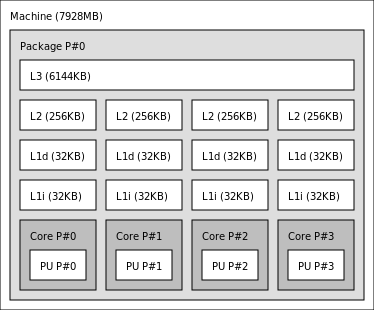
\includegraphics[width=0.5\columnwidth]{./opti7020-topo.png}
  \caption{Topology information of a Dell OptiPlex 7020}
\end{figure}

\newpage

\subsection{Timing Results}
In the following tables and plots the recorded execution times are displayed.

%------------------------------------ 1

\begin{table}[htbp]
  \centering
    \begin{tabular}{|c c||l l l l| l|} 
    \hline
    \multicolumn{7}{|c|}{Timing results of matrix multiplication (Time unit: seconds)} \\
    \multicolumn{7}{|c|}{Array size: 1024x1024} \\
    \hline
    \# of nodes & \# of processes & 1st run & 2nd run & 3rd run & 4th run & Average time\\ [0.5ex] 
    \hline\hline
    2 & 8 & 1.796173 & 1.677769 & 1.640642 & 1.744993 & 1.71489425 \\ 
    \hline
    4 & 16 & 1.281953 & 1.165645 & 1.255963 & 1.188320 & 1.22297025 \\
    \hline
    8 & 32 & 1.077676 & 1.080606 & 1.104992 & 1.100065 & 1.09083475 \\ [1ex]
    \hline
    \end{tabular}
  \caption{Timing results of 2D matrix multiplication}
\end{table}


\begin{figure}[htbp]
  \centering
  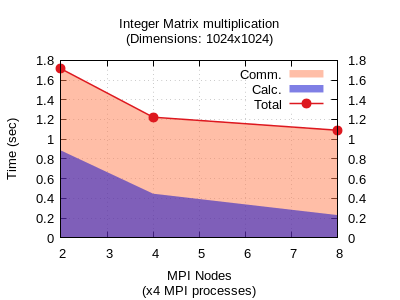
\includegraphics[width=0.55\columnwidth]{../../hw3/ex1/plots/matmul.png}
  \caption{Timing results of 2D matrix multiplication}
\end{figure}

%------------------------------------


\subsection{Conclusion}
Based on the results presented above and given that the average execution time of the serial
program is 3,79148025 seconds, we conclude that:

\begin{itemize}
 \item Program performance is increased as the number of nodes is increased. A speedup of
       about 2.2 and 3.5 times is achieved in the worst and best case correspondingly.
 \item Even though communication overheads are introduced the time spent in calculations
       is halved proportionally to the number of nodes, while the time spent in communications
       slightly increases. For this reason it is safe to conclude that the speedup is
       achieved due to the significant speedup in calculation time.
\end{itemize}

\newpage

%+----------------------------------------------------------+
%|                                                          |
%|          EXERCISE #2                                     |
%|                                                          |
%+----------------------------------------------------------+

\section{Exercise \#2}

\subsection{About}
This exercise is about the multiplication of integer $N$x$N$ arrays using \texttt{MPI},
\texttt{OpenMP} and strip-partitioning. This hybrid programming model means to take
advantage of the best features of the distributed and shared-memory programming models.
\texttt{MPI} is used to distribute work between nodes while \texttt{OpenMP} is used to
achieve parallelization over each node. The purpose of this exercise is the same
as in Exercise \#1.

\subsection{Experiment details}
During this experiment, \texttt{MPI} node number takes value in \{2, 4, 8\}, 1 \texttt{MPI}
process \& 4 \texttt{OpenMP} threads run on each node and array size is 1024x1024.

\subsubsection{System Specifications}
The experiments were conducted again on a cluster of Dell OptiPlex 7020s.

\subsection{Timing Results}
In the following tables and plots the recorded execution times are displayed.

%------------------------------------ 1

\begin{table}[htbp]
  \centering
    \begin{tabular}{|c c||l l l l| l|} 
    \hline
    \multicolumn{7}{|c|}{Timing results of matrix multiplication (Time unit: seconds)} \\
    \multicolumn{7}{|c|}{Array size: 1024x1024} \\
    \hline
    \# of nodes & \# of processes & 1st run & 2nd run & 3rd run & 4th run & Average time\\ [0.5ex] 
    \hline\hline
    2 & 2 & 1.409800 & 1.487245 & 1.398054 & 1.433354 & 1.43211325 \\ 
    \hline
    4 & 4 & 1.336848 & 1.319516 & 1.368628 & 1.422378 & 1.3618425 \\
    \hline
    8 & 8 & 1.352629 & 1.279406 & 1.268784 & 1.254344 & 1.28879075 \\ [1ex]
    \hline
    \end{tabular}
  \caption{Timing results of 2D matrix multiplication}
\end{table}


\begin{figure}[htbp]
  \centering
  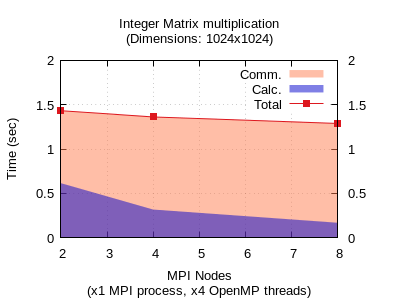
\includegraphics[width=0.55\columnwidth]{../../hw3/ex2/plots/matmul.png}
  \caption{Timing results of 2D matrix multiplication}
\end{figure}

%------------------------------------
\pagebreak

\subsection{Conclusion}
Based on the results presented above and given that the average execution time of the serial
program is 3,79148025 seconds, we conclude that:

\begin{itemize}
 \item Increasing the number of \texttt{MPI} nodes lead in a linear decrease
       of the time spent in calculations, while the time spend in communications
       increases and almost leads to a negligible speedup. As a result, the overall
       execution time remains almost constant with speedup varying between 2.5 and 3 times.
\end{itemize}


%+----------------------------------------------------------+
%|                                                          |
%|          EXERCISE #3                                     |
%|                                                          |
%+----------------------------------------------------------+

\section{Exercise \#3}

\subsection{About}
This exercise is about the calculation of the mathematical constant $\pi$ using \texttt{MPI}
and dynamic scheduling. During dynamic scheduling the parallelizable loops are divided
into chunks of iterations (tasks) and are dispatched to the processes available for execution.
The dispatch takes place in respect to the current processor workload where each process executes
and as a result load balancing is achieved. The purpose of this exercise is to time the calculation
of $\pi$ and observe how altering the number of \texttt{MPI} nodes will affect execution time
and what amount of this time is spent in communications.


\subsection{Experiment details}
The calculation consists of $N*10^3$ loop iterations, where N is the number of tasks provided
by the user during runtime and $10^3$ is the chunksize. Finally, node number takes value in
\{2, 4, 8\}.

\subsubsection{System Specifications}
The experiments were conducted once again on a cluster of Dell OptiPlex 7020s.

\subsection{Timing Results}
In the following tables and plots the recorded execution times are displayed.

%------------------------------------ 1

\begin{table}[htbp]
  \centering
    \begin{tabular}{|c c||l l l l| l|} 
    \hline
    \multicolumn{7}{|c|}{Timing results of $\pi$ calculation (Time unit: seconds)} \\
    \hline
    \# of nodes & \# of processes & 1st run & 2nd run & 3rd run & 4th run & Average time\\ [0.5ex]
    \hline\hline
    2 & 8 & 0.134720 & 0.135512 & 0.138103 & 0.133741 & 0.135519 \\ 
    \hline
    4 & 16 & 0.107681 & 0.111158 & 0.110939 & 0.109459 & 0.10980925 \\
    \hline
    8 & 32 & 0.088115 & 0.088238 & 0.087841 & 0.088177 & 0.08809275 \\ [1ex]
    \hline
    \end{tabular}
  \caption{Timing results of $\pi$ calculation}
\end{table}


\begin{figure}[htbp]
  \centering
  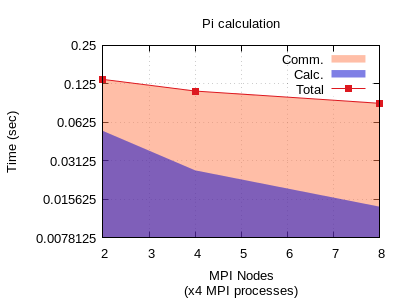
\includegraphics[width=0.55\columnwidth]{../../hw3/ex3/plots/pi.png}
  \caption{Timing results of $\pi$ calculation}
\end{figure}

\newpage
\subsection{Conclusion}
Based on the results presented above and given that the average execution time of the serial
program is 0.385222 seconds, we conclude that:

\begin{itemize}
 \item Using \texttt{MPI} leads to execution times at least four (4) times bigger compared
       to the one of the serial program and keeps increasing proportionally to the number
       of nodes.
 \item Although the time spent in calculations is decreased and the speed up achieved
       exceeds 200 times, the huge communication overheads result in an increase of the total
       execution time.
\end{itemize}

\end{document}